\documentclass[tikz,border=2pt]{standalone}
\usepackage{amsmath}
\usetikzlibrary{arrows.meta}
\begin{document}
% (Q,r) policy with Q = 3, r = 0: the inventory position cycles through 1, 2, 3. With
% f_i = P(D = i mod 3), it stays with prob f_0, moves one level down cyclically with f_1 and two
% levels down with f_2; every state receives f_0 + f_1 + f_2 = 1, so p(i) = 1/3.
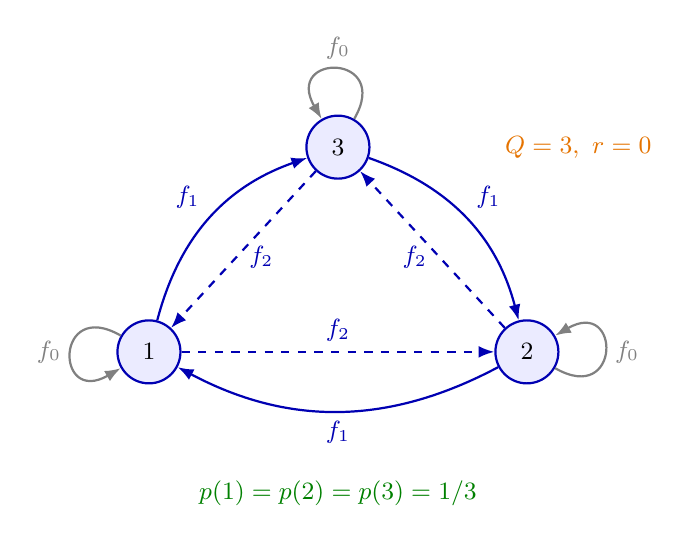
\begin{tikzpicture}[font=\small, >={Latex[length=2mm]},
  state/.style={circle, draw=blue!70!black, fill=blue!8, thick, minimum size=8mm}]
  \node[state] (s3) at (0,2.6) {$3$};
  \node[state] (s2) at (2.4,0) {$2$};
  \node[state] (s1) at (-2.4,0) {$1$};
  % one level down (f_1), drawn outside
  \draw[->, blue!70!black, thick] (s3) to[bend left=28] node[above right] {$f_1$} (s2);
  \draw[->, blue!70!black, thick] (s2) to[bend left=28] node[below] {$f_1$} (s1);
  \draw[->, blue!70!black, thick] (s1) to[bend left=28] node[above left] {$f_1$} (s3);
  % two levels down (f_2), drawn inside as straight chords
  \draw[->, blue!70!black, thick, dashed] (s3) -- node[pos=0.55, right, xshift=1pt] {$f_2$} (s1);
  \draw[->, blue!70!black, thick, dashed] (s1) -- node[pos=0.5, above] {$f_2$} (s2);
  \draw[->, blue!70!black, thick, dashed] (s2) -- node[pos=0.45, left, xshift=-1pt] {$f_2$} (s3);
  % self-loops (f_0)
  \draw[->, gray, thick] (s3) to[out=60, in=120, looseness=6] node[above] {$f_0$} (s3);
  \draw[->, gray, thick] (s2) to[out=-30, in=30, looseness=6] node[right] {$f_0$} (s2);
  \draw[->, gray, thick] (s1) to[out=150, in=210, looseness=6] node[left] {$f_0$} (s1);
  \node[orange!90!black, anchor=west] at (2.0,2.6) {$Q=3,\ r=0$};
  \node[green!50!black] at (0,-1.8) {$p(1)=p(2)=p(3)=1/3$};
\end{tikzpicture}
\end{document}
